
\subsection{Process Layer}\label{subsec:process_layer}
%\addcontentsline{toc}{subsection}{Process Layer}
The Process Layer specifies the interactions taking place between the different components of the International Data Spaces. It thereby provides a dynamic view of the Reference Architecture Model. 

In the following, three major processes and their sub processes are described:



\begin{enumerate}
	\item \textbf{Onboarding,}  i.e. what to do to be granted access to the International Data Spaces as a Data Provider or Data User;

	\item \textbf{Exchanging data,} i.e. searching for a suitable Data Provider and invoking the actual data operation; and

	\item \textbf{Publishing and using Data Apps, }i.e. interacting with the IDS as an App Provider and user of a Data App, respectively.

\end{enumerate}\par



These three processes are related to the International Data Space's key value propositions and involve most of the roles introduced in the Business Layer section. The processes are illustrated using the Business Process Modeling Notation (BPMN).


\subsubsection{Onboarding}
%\addcontentsline{toc}{subsubsection}{Onboarding}
The overall $``$Onboarding$"$  process consists of several sub processes. The first step for an organization to join the International Data Spaces as a Data Provider or Data User is to acquire an identity to be used in the IDS. This identity, which forms the basis for establishing trusted communication in the IDS, is provided by the Certification Body and an Evaluation Facility in the form of a certificate issued by an Identity Provider. In a second step, the organization needs to request a Connector from a Software Provider. The Connector, being the core technical component for becoming part of the IDS, must then be installed. After that, it receives a digital certificate (X.509 certificate) to make sure it complies with IDS specifications and requirements. The digital certificate is based on the certification of the participant and the certification of the Connector (see section 3.1 and section 4.2).  In a third step, the Connector needs to be configured for internal use and prepared for secure communication ("Security Setup", see below). In the final step, the Connector needs to be made available for other participants in the IDS so that it can finally enter live operation. 
%ToDo referer

The overall $``$Onboarding$"$  process is illustrated in Figure \ref{fig:_Overall_onboarding_process}.The following paragraphs describe each step of the onboarding process in more detail.

%ToDo:update figure
%%%%%%%%%%%%%%%%%%%% Figure/Image No: 14 starts here %%%%%%%%%%%%%%%%%%%%

\begin{figure}[H]
	\begin{Center}
		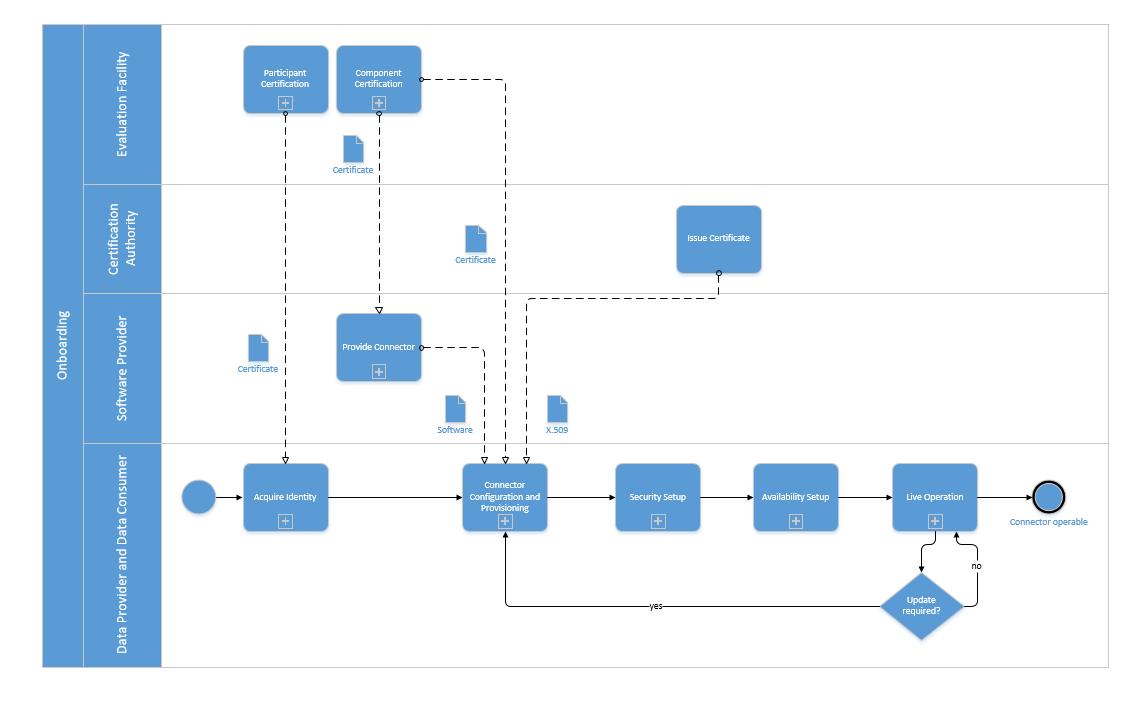
\includegraphics[width=6.53in,height=2.74in]{./media/image22.PNG}
		\caption{ $``$Onboarding$"$  overall process}
		\label{fig:_Overall_onboarding_process}
	\end{Center}
\end{figure}


%%%%%%%%%%%%%%%%%%%% Figure/Image No: 14 Ends here %%%%%%%%%%%%%%%%%%%%


\textbf{Acquire Identity}

Any organization that wants to operate a connector in order to exchange data in the International Data Spaces as a Data provider or Data Consumer needs to acquire a unique identity in the form of a certificate. This certificate enables them to establish secure and trusted connections to other IDS participants (see section 3.1).


\textbf{Connector Configuration and Provisioning}

Each Connector that participates in the IDS ecosystem must provide a self-description for other IDS participants to read, expressed in terms of the Information Model (see section 3.4). The respective organization needs to create this description at the beginning of the connector configuration and provisioning sub process. The Connector self-description must contain information about the respective organization, about who maintains the Connector (i.e. the Service Provider), and about the content and type of the data offered or requested.

Another mandatory step for the organization to take is to orchestrate data flows for (future) data retrieval and data provisioning, respectively, and to set up system adapters and communication interfaces ("endpoints"). (Details on the configuration of the IDS Connector are described in section 3.5.1.1.)

If needed, the organization can install and configure Data Apps acquired from the App Store.


%%%%%%%%%%%%%%%%%%%% Figure/Image No: 14 starts here %%%%%%%%%%%%%%%%%%%%

\begin{figure}[H]
	\begin{Center}
		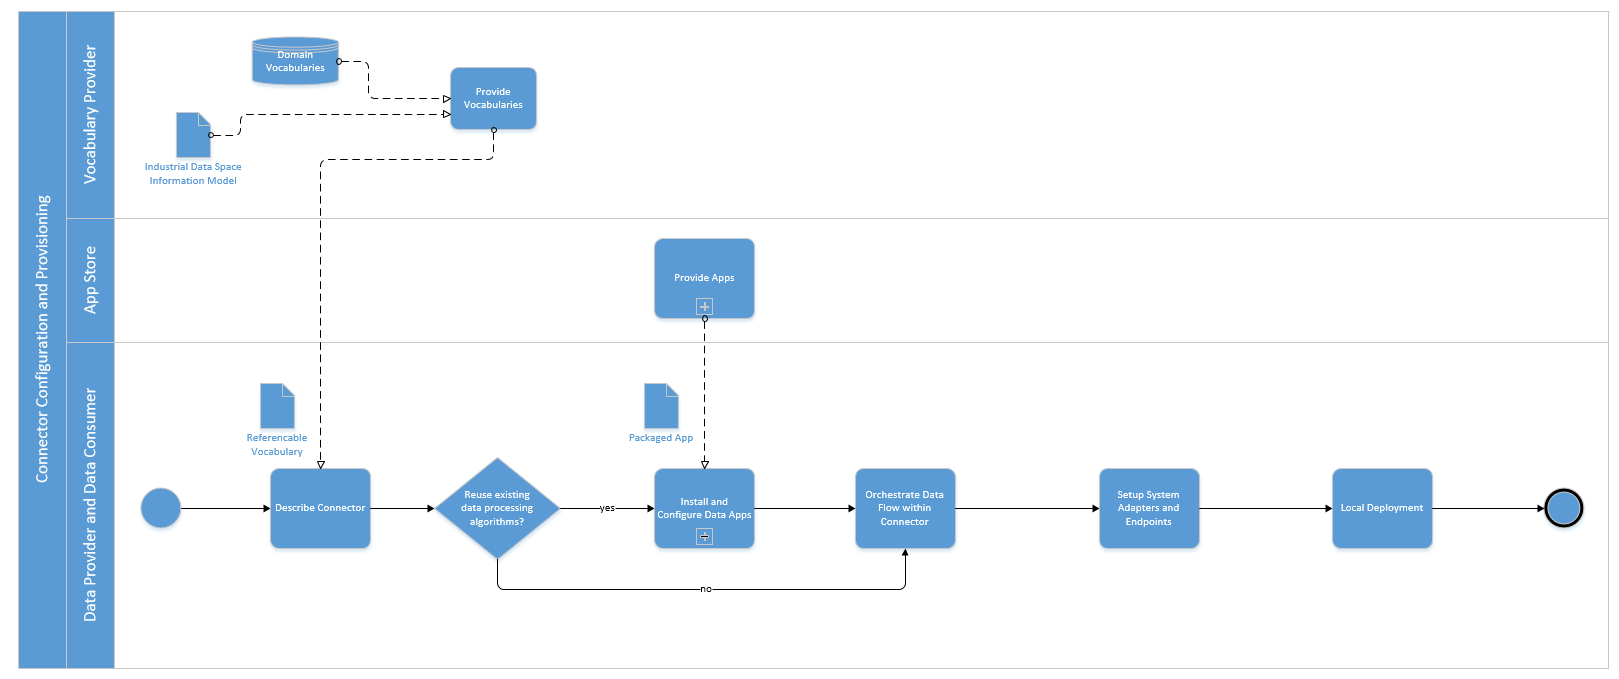
\includegraphics[width=6.53in,height=2.74in]{./media/image23.PNG}
		\caption{ $``$Connector Configuration and Provisioning$"$  sub process}
		\label{ fig:_Connector_Configuration_and_Provisioning_sub_process}
	\end{Center}
\end{figure}


%%%%%%%%%%%%%%%%%%%% Figure/Image No: 14 Ends here %%%%%%%%%%%%%%%%%%%%

\textbf{Security Setup}

To enable secure communication, a Certification Authority issues a certificate to the Data Provider or Data Consumer. This certificate is deployed locally to enable Transport Layer Security (TLS) and identification of the respective IDS participant. On top of that, the Connector self-description must be correct and valid, which is ensured by requesting a Dynamic Attribute Token from the Identity Provider (section 4.1). The token is a signed attestation that the information the Connector states about itself has been verified and is actually true. The token is presented by each subsequent outgoing communication message of the Connector, so that also the communicating Connectors have a means to verify the trustfulness of their communication partners at any time.

Furthermore, any organization that wants to assume the role of Data Provider or Data Consumer has the option to configure custom access restrictions for bilateral communications. For instance, a Data Provider may want to block certain Connectors or participants from accessing their services, or it may require specific access credentials. These configurations may be set up in the last step of the Security Setup sub process (see section 4.1).



%%%%%%%%%%%%%%%%%%%% Figure/Image No: 15 starts here %%%%%%%%%%%%%%%%%%%%

\begin{figure}[H]
	\begin{Center}
		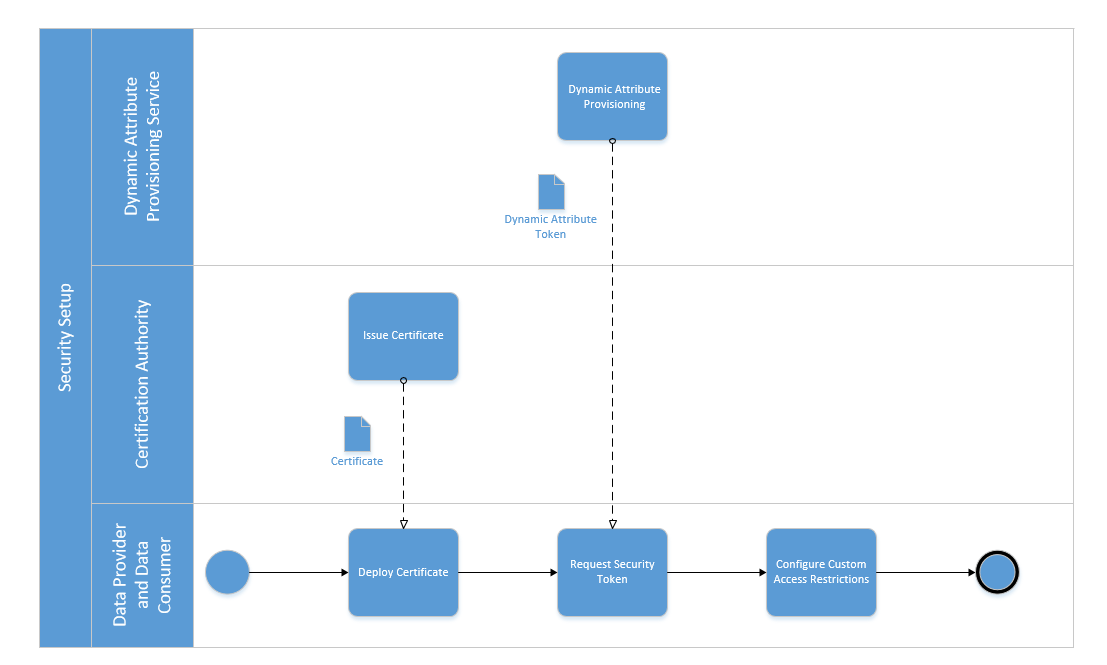
\includegraphics[width=7.03in,height=4.22in]{./media/image24.png}
		\caption{$``$Security Setup$"$  sub process}
		\label{fig:Security_Setup_sub_process}
	\end{Center}
\end{figure}


%%%%%%%%%%%%%%%%%%%% Figure/Image No: 15 Ends here %%%%%%%%%%%%%%%%%%%%

% check for Figure : \par


\textbf{Availability Setup}

After local Connector deployment and Security Setup, a Connector must be made available for other participants in the International Data Spaces. This is done by the provisioning of an $``$External Connector$"$ , which runs in a so-called $``$Demilitarized Zone (DMZ)$"$  and forwards or filters requests to the $``$Internal Connector$"$ . Alternatively, proper adjustment of firewall rules may be sufficient (in less sensitive environments). Each Data Provider and Data Consumer can decide whether or not they want to announce their Connector (or the data resources accessible through their Connector) publicly on the IDS. If they do so, they can select a Broker from a set of available Broker services (i.e., a registry for Connector self-descriptions) to publish the self-description of their Connector (see above). The Broker provides functions for searching for and retrieving registered Connector self-descriptions (see section 3.5.2), including data sources, interfaces, security profiles, and current levels of trustworthiness.



%%%%%%%%%%%%%%%%%%%% Figure/Image No: 16 starts here %%%%%%%%%%%%%%%%%%%%

\begin{figure}[H]
	\begin{Center}
		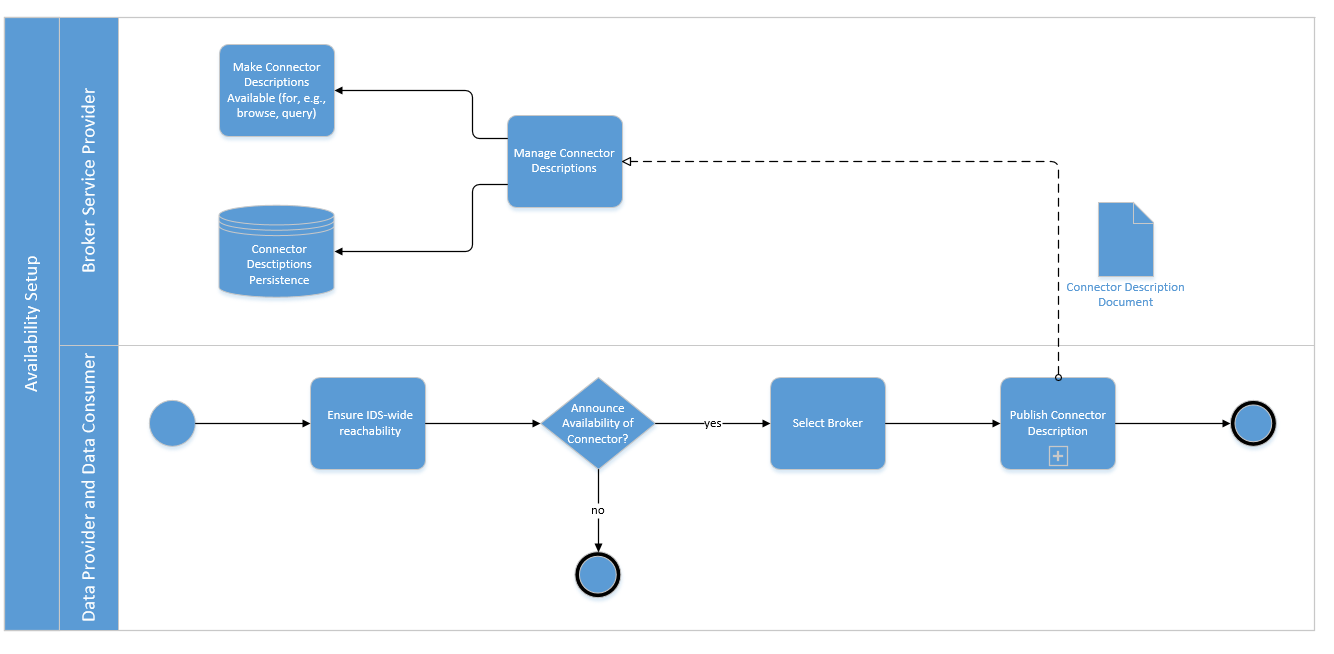
\includegraphics[width=6.25in,height=3.06in]{./media/image25.png}
		\caption{$``$Availability Setup$"$  sub process}
		\label{fig:Availability_Setup_sub_process}
	\end{Center}
\end{figure}


%%%%%%%%%%%%%%%%%%%% Figure/Image No: 16 Ends here %%%%%%%%%%%%%%%%%%%%



\subsubsection{Exchanging Data}
%\addcontentsline{toc}{subsubsection}{Exchanging Data}
The overall process of exchanging data consists of two sub processes, as illustrated in Figure \ref{fig:_Exchanging_Data__overall_process_}. The first sub process is about a Data Consumer searching for a suitable Data Provider. If the search was successful, the Data Consumer and the Data Provider can start to exchange data with one another. This is done after Connector configuration, either starting "from scratch" (see IDS onboarding process described above) or by reconfiguring an existing Connector. The second sub process is the invocation of the actual data operation (e.g. data upload or download, data transformation, or data query).

%%%%%%%%%%%%%%%%%%%% Figure/Image No: 17 starts here %%%%%%%%%%%%%%%%%%%%

\begin{figure}[H]
	\begin{Center}
		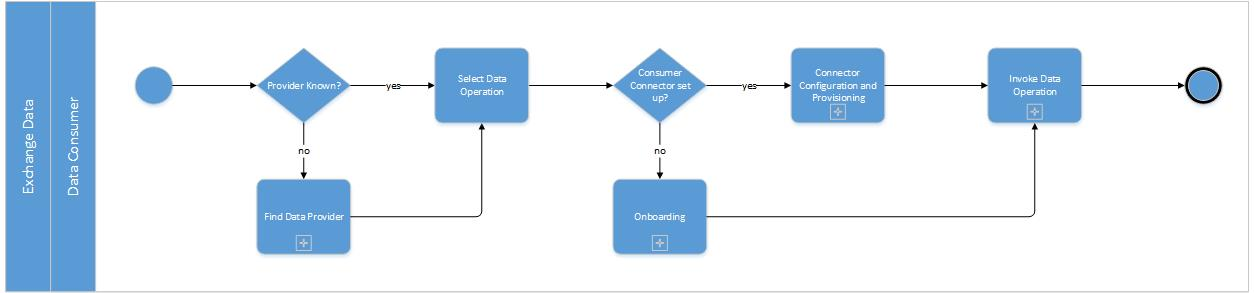
\includegraphics[width=6.53in,height=1.53in]{./media/image26.jpeg}
		\caption{ $``$Exchanging Data$"$  overall process }
		\label{fig:_Exchanging_Data__overall_process_}
	\end{Center}
\end{figure}


%%%%%%%%%%%%%%%%%%%% Figure/Image No: 17 Ends here %%%%%%%%%%%%%%%%%%%%


\textbf{Find Data Provider}

To find a Data Provider, the Data Consumer must send a query to a Broker Service Provider. Before that, however, the Data Consumer needs to select a suitable Broker (e.g. based on thematic coverage) and determine the query capabilities (e.g. a graphical search interface or a domain-specific query language). The Broker then returns the query result to the Data Consumer, who needs to interpret the result to find out about the different data sources available in the International Data Spaces for providing the data specified in the query. Each query result must provide information about each IDS Connector capable of providing the desired data, so that the Data Consumer can retrieve each Connector's self-description to learn more about how to receive the desired dataset from a technical point of view (e.g., endpoint addresses, protocol). The Data Provider may serve the same data using different representations or pricing options, so the Data Consumer may select a suitable offer from the Data Provider's Connector description.

Alternatively, the Data Consumer may already know a suitable Data Provider. In this case, the Data Consumer can contact the Data Provider directly (i.e. without invoking a broker).



%%%%%%%%%%%%%%%%%%%% Figure/Image No: 18 starts here %%%%%%%%%%%%%%%%%%%%

\begin{figure}[H]
	\begin{Center}
		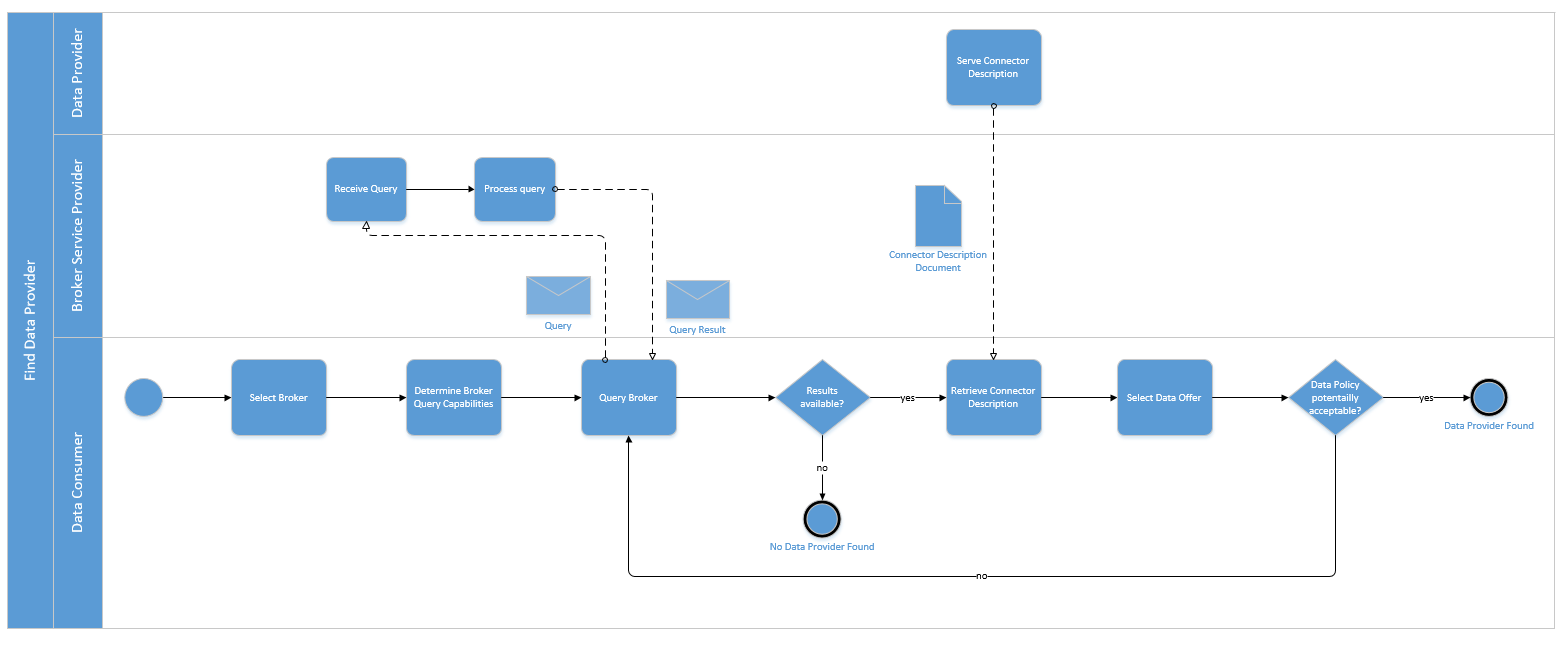
\includegraphics[width=6.53in,height=2.74in]{./media/image27.PNG}
		\caption{ $``$Find Data Provider$"$  sub process}
		\label{fig:_Find_Data_Provider__sub_process}
	\end{Center}
\end{figure}


%%%%%%%%%%%%%%%%%%%% Figure/Image No: 18 Ends here %%%%%%%%%%%%%%%%%%%%



\textbf{Invoke Data Operation}

Data usage policy information is an important element of legal agreements and is therefore modeled as first-class objects on the Information Layer (see Section 3.4). The handling of data usage policy information is shown in detail in the $``$Invoke Data Operation$"$  sub process (Figure \ref{fig:invole_data_operation}). While a Connector self-description basically contains information about the datasets available, also usage policy information can be extracted from this description. In a (semi-)automated negotiation process performed by the usage control frameworks of the participating Connectors, the Data Consumer and the Data Provider need to agree on a data usage policy. If an agreement has been reached, this policy is instantiated and deployed inside both Connectors. The policy both parties agree upon needs to be persisted in an immutable way by both sides. After the data usage policy has been established, the consuming Connector can be configured to deal with further data coming in from the Data Provider in the future as specified by the policy. The retrieval of the self-description and the negotiation of policies must make use of HTTPS or mqtt protocols. If this has been done, the Data Operation call can be invoked – this is usually done by a request using a common protocol (e.g., HTTP) to retrieve a data artifact from the Data Provider. 

The Data Provider then sends the result of the data operation to the Data Consumer. Usage control on both sides signals the data operation to the data provenance tracking infrastructure (accessible via the Clearing House), so that provenance information about the data transferred is kept up to date. Usage control on the Data Consumer side also signals receipt of the data operation result to the data provenance tracking infrastructure, in order to confirm that the transaction has been completed successfully (see sections 4.1.3.6 and 4.1.3.7). 


%%%%%%%%%%%%%%%%%%%% Figure/Image No: 19 starts here %%%%%%%%%%%%%%%%%%%%

\begin{figure}[H]
	\begin{Center}
		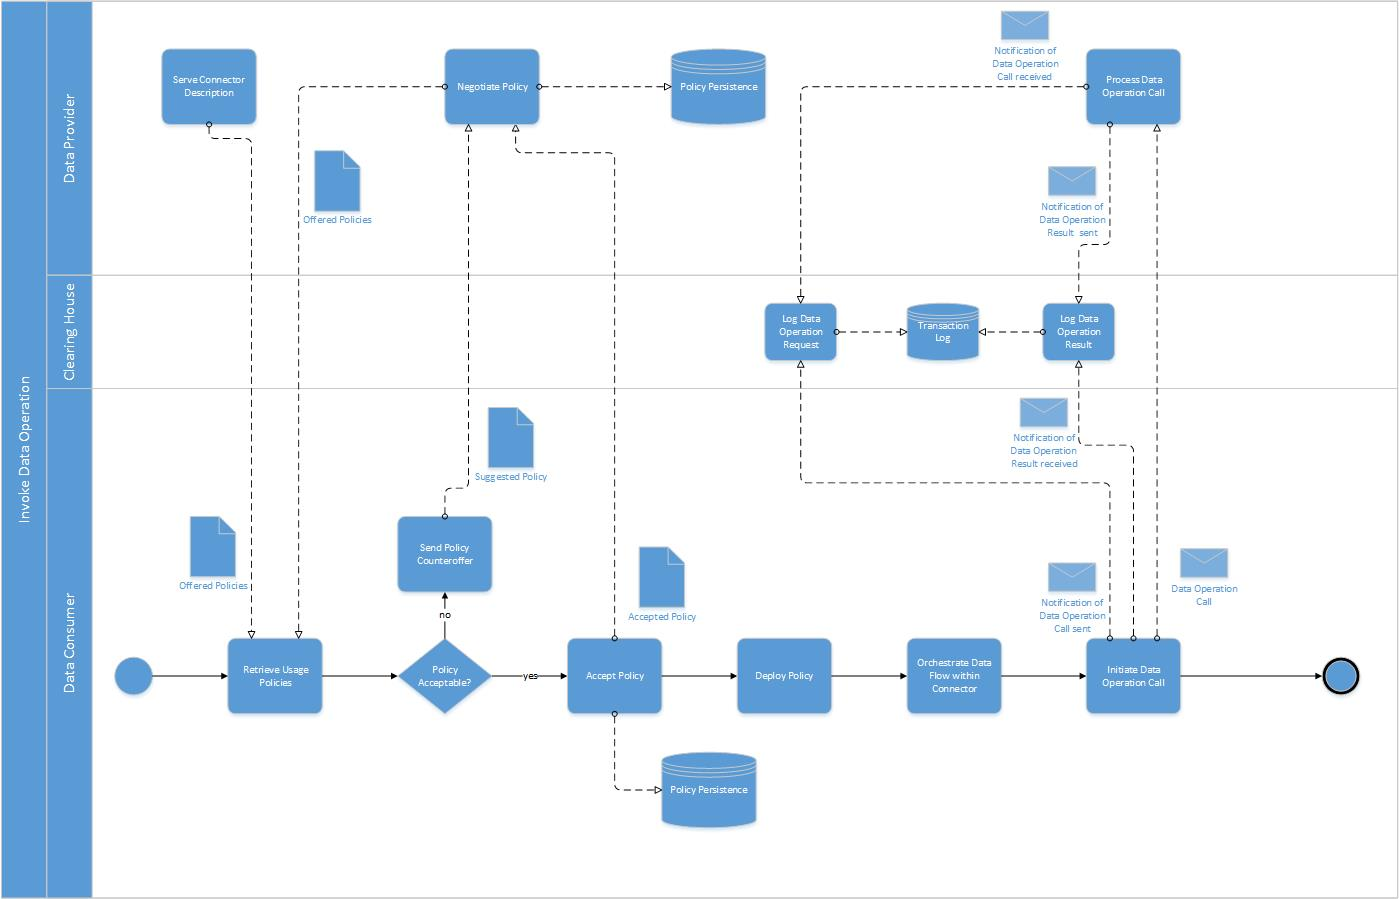
\includegraphics[width=6.53in,height=4.2in]{./media/image28.jpeg}
		\caption{$``$Invoke Data Operation$"$  sub process	}
		\label{fig:invole_data_operation}
	\end{Center}
\end{figure}


%%%%%%%%%%%%%%%%%%%% Figure/Image No: 19 Ends here %%%%%%%%%%%%%%%%%%%%

Communication between the Connectors can be asynchronous (i.e., the Data Consumer does not have to wait in idle mode for the result to arrive, but will be notified by the Data Provider as soon as the result is available). Instead of a pull-request, a push-request can be sent, which means that the Data Consumer asks for updates regarding the requested data. The updated data can be provided either after certain events (e.g., after the data has been updated by the Data Provider) or within certain time intervals (e.g., every five minutes). If a push-request is made, the Data Consumer repeatedly receives updated query results from the Data Provider. In case of a pull-request, the Data Consumer can repeat the last part of the process to query data again (using the same or a different query). The description of the communication pattern itself is not part of this document, as this is covered by existing standards (e.g. DIN SPEC 16593-1:2018-04, see chapter 8 $``$Characterizations of Interactions$"$ ) or as best practices in industry. 
		


\subsubsection{Publishing and Using Data Apps}
%\addcontentsline{toc}{subsubsection}{Publishing and Using Data Apps}
Data Apps can be used by Connectors for specific data processing or data transformation tasks. They can perform tasks of different complexity, ranging from simple data transformation to complex data analytics. An example of data transformation may be a Data App parsing a single string field with address information and producing a data structure consisting of street name and number, zip code, name of the city, and name of the country.\\
On a conceptual level, Data Apps can be treated the same way as data offerings in the International Data Spaces. Therefore, just as data is provided by a Data Provider using a Connector and registering this Connector at a Broker, Data Apps are created by an App Provider and registered at an App Store (using the App Provider's Connector as a means to communicate with the App Store). As a consequence, App Providers also need to undergo the Onboarding process. However, instead of registering their Connector at a Broker, App Providers register their Data Apps at an App Store.\\
In order to be published, certain Data Apps require certification from the Certification Body (see section 3.5.1) (see first step of the process shown in Figure \ref{fig:_Data_App_Certification__process}).



%%%%%%%%%%%%%%%%%%%% Figure/Image No: 20 starts here %%%%%%%%%%%%%%%%%%%%

\begin{figure}[H]
	\begin{Center}
		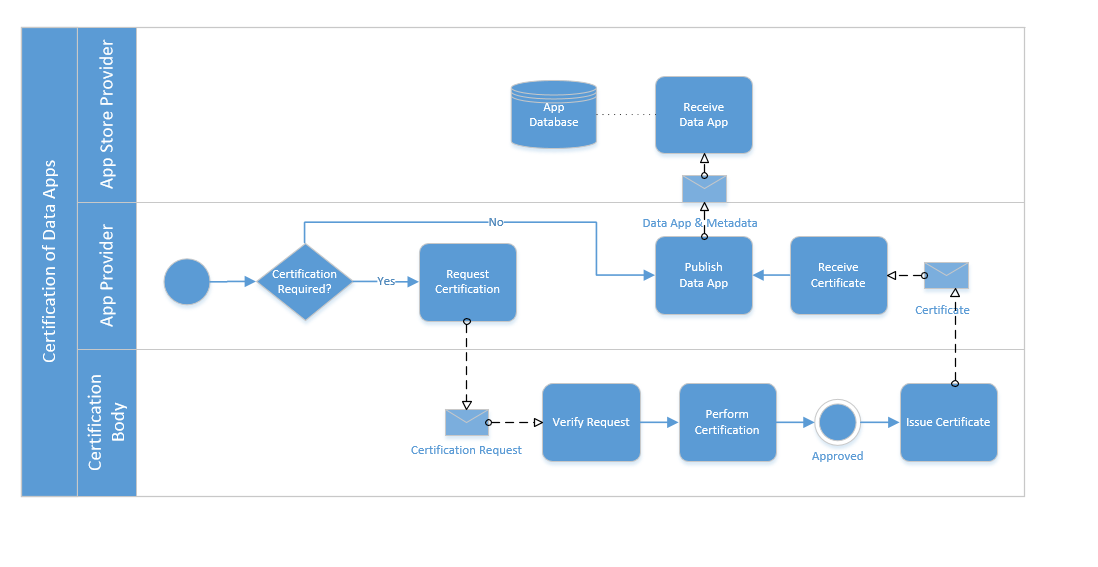
\includegraphics[width=6.47in,height=3.34in]{./media/image29.png}
		\caption{ $``$Data App Certification$"$  process}
		\label{fig:_Data_App_Certification__process}
	\end{Center}
\end{figure}


%%%%%%%%%%%%%%%%%%%% Figure/Image No: 20 Ends here %%%%%%%%%%%%%%%%%%%%



%%%%%%%%%%%%%%%%%%%% Figure/Image No: 21 starts here %%%%%%%%%%%%%%%%%%%%

\begin{figure}[H]
	\begin{Center}
		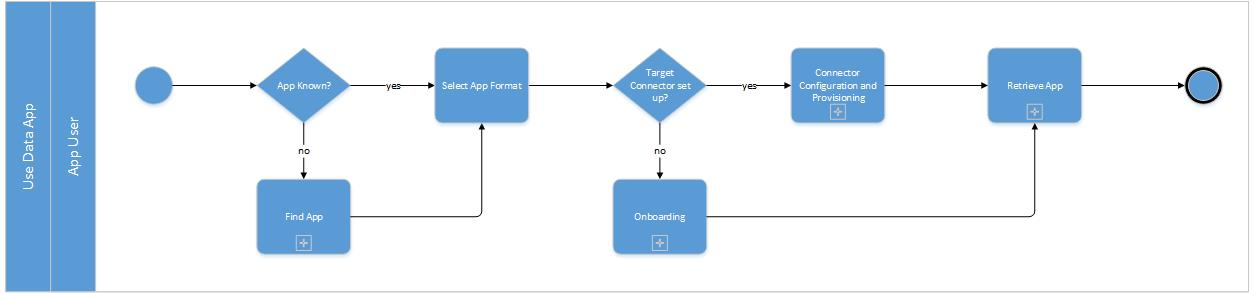
\includegraphics[width=6.53in,height=1.53in]{./media/image30.jpeg}
		\caption{Use Data App process}
		\label{fig:use_data_app}
	\end{Center}
\end{figure}
%%%%%%%%%%%%%%%%%%%% Figure/Image No: 21 Ends here %%%%%%%%%%%%%%%%%%%%

When it comes to using a Data App that is offered by an App Store, App Users (Data Provider or Data Consumer) need to execute a process that is very similar to the $``$Exchange Data$"$  process described above.
For each Data App that was successfully certified, the corresponding metadata is stored in the App Store for being retrieved by users (e.g., Data Consumers or Data Providers) via a search interface. Searching for a Data App is part of the “Find App” sub process depicted in Figure \ref{fig:use_data_app}. If a user finds a suitable Data App (i.e., matching in functionality and compatible with the user’s Connector packaging format) in the App Store, the App can be requested. This is indicated in the “Retrieve App” sub process, which is conceptually identical with the “Invoke Data Operation” process outlined in section 3.3.2, which is why a detailed discussion is omitted here.

